\documentclass[16pt, a4paper]{article}
\usepackage[T1,T2A]{fontenc}
\usepackage[utf8]{inputenc}
\usepackage[english,russian]{babel}
\usepackage{graphicx}
\usepackage{wrapfig}
\usepackage{amsmath,amsthm,amssymb}
\usepackage{fancyhdr}
\usepackage{lastpage}
\usepackage{ifthen}
\usepackage{geometry}
\geometry{a4paper,top=2cm,bottom=2cm,left=2cm,right=2cm}

\pagestyle{fancy}
\fancyhead[R]{}
\fancyhead[L]{}
\fancyhead[C]{\ifthenelse{\isodd{\thepage}}{\textbf{\Large{Научно-исследовательская работа}}}{\textbf{\Large{Исследование эволюции вещества после соударения тяжелых ультрарелятивистских ионов}}}}
\renewcommand{\headrulewidth}{0.7 mm}
\setlength{\headheight}{31pt}

\fancyfoot[R]{\Large{\textbf{\LaTeX}}}
\fancyfoot[L]{\large{\textbf{Страница \thepage \ из \pageref{LastPage}}}}
\fancyfoot[C]{}
\renewcommand{\footrulewidth}{0.7 mm}

\title{\textbf{Исследование эволюции вещества после соударения тяжелых ультрарелятивистских ионов}}
%\author{Лопатин Даниил}
\date{October 2022}

%------------------------------------------------------------------------------------
%\begin{figure}[h!]
    %\center{\includegraphics[width=1\linewidth]{12.PNG}}
    %\caption{Зависимость сигнала от шума для данных.}
    %\label{ris:image}
%\end{figure}

%\begin{wrapfigure}[18]{l}{0.4\linewidth} 
    %\vspace{-5ex}
    %\includegraphics[width=\linewidth]{4}
    %\caption{Some caption}
    %\label{fig:somelabel}
%\end{wrapfigure}

%------------------------------------------------------------------------------------

\begin{document}

\maketitle
\thispagestyle{fancy}

\subsection*{Теория}

Рассмотрим скалярную теорию поля с лагранжианом

$$ \mathcal{L} = \frac12\dot{\varphi}^2 - \frac\lambda 4\varphi^4 + J\varphi $$

Уравнение движения

$$ \ddot{\varphi} + \frac\lambda 6\varphi^3 - J = 0 \eqno(1) $$

Точное решение 

$$ \varphi(t) = \varphi_{max}cn\Big(\frac12;\sqrt{\frac\lambda 6}\phi_{max}(t-t_0)+C\Big), $$

где $cn$ - эллиптическая функция Якоби.

Рассмотрим эволюцию тензора энергии-импульса

$$ T^{\mu\nu} = \partial^\nu\varphi\partial^\nu\varphi - g^{\mu\nu}\Big(\frac12\partial_\sigma\varphi\partial^\sigma\varphi-\frac\lambda{24}\varphi^4\Big) $$

Представляется интересной возможность достижения "гидродинамического" режима
$\varepsilon = 3p$

$$ \varepsilon_0 = \frac{\dot{\varphi}^2}{2} + \frac{\lambda\varphi^4}{24},\,\,\,\,\,\,p_0 =  \frac{\dot{\varphi}^2}{2} - \frac{\lambda\varphi^4}{24}, $$

где $\varphi = \varphi_0$ - решение уравнения движения (1).

Получившаяся динамика энергии и давления предсавлена на рисунке...

Проведем усреднение по начальным условиям. После некоторого временного 
периода получаем точно определяемое уравнение состояния.

\begin{wrapfigure}[20]{l}{0.55\linewidth} 
    %\vspace{-5ex}
    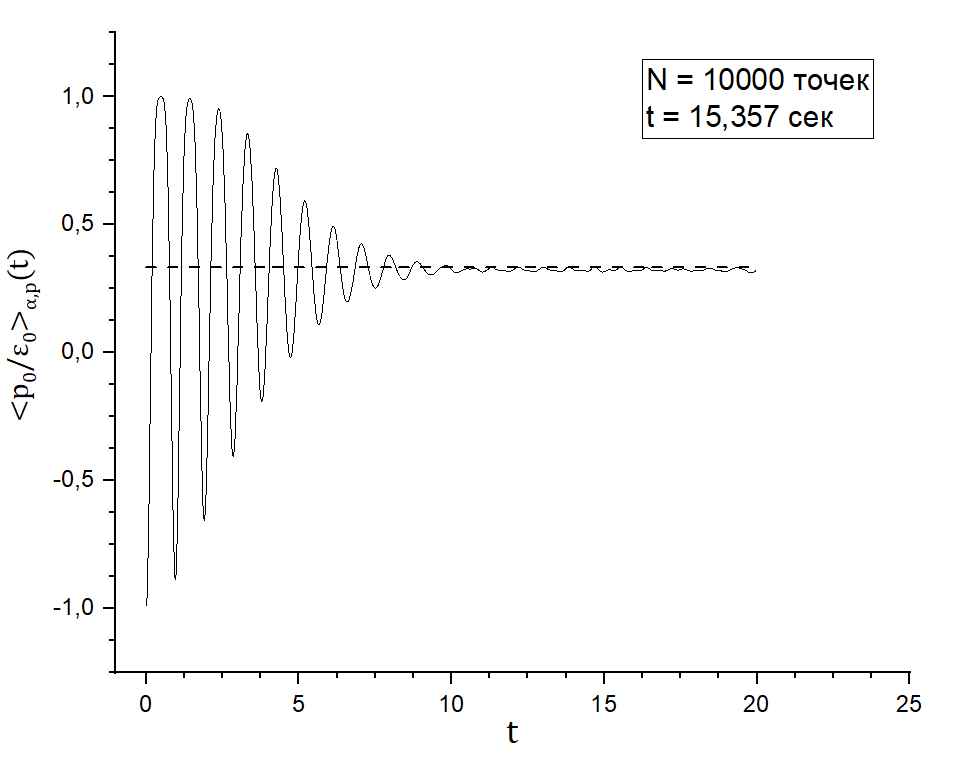
\includegraphics[width=1\linewidth]{3.PNG}
    %\caption{Some caption}
    %\label{fig:somelabel}
\end{wrapfigure}

Усреднение по начальным данным проводим с использованием функции Вигнера

$$ f_W(\alpha, p, 0) = \frac{1}{\alpha_0p_0\pi}e^{-\frac{(\alpha-A)^2}{\alpha_0^2}-\frac{p^2}{p_0^2}}, $$

где $A$ - начальная амплитуда поля, а $\alpha_0$ и $p_0$ - нормировочные константы.

Таким образом, мы считаем интеграл

$$ \iint f_W(\alpha, p, 0)\,\varphi(\alpha, p, t) \,d\alpha\,dp $$

\hspace{14pt}

\subsection*{Экспериментальная установка}

\subsection*{Ход работы}

\begin{enumerate}
    \item 

    \item
    
\end{enumerate}

\end{document}